%% Adapted from GaTech CS 7545 Machine Learning Theory given by Prof. Jacob Abernathy Fall 2018. Original latex file: https://github.com/mltheory/CS7545/blob/master/scribe/CS7545scribe_template.tex 



%%%%%PLEASE CONSIDER CORRECTIONS AT PLACES INDICATED%%%%%%%%
\documentclass{article}
%%%%%Packages Used, add more if necessary%%%%
\usepackage{amsmath,amsfonts,amssymb,graphicx,fullpage, float}
\setlength{\topmargin}{-0.6 in}
\setlength{\textheight}{8.5 in}
\setlength{\headsep}{0.75 in}
\usepackage{mdframed}
\usepackage{multicol}
\usepackage{microtype, hyperref}


%%%%% NO NEED TO EDIT THIS PREAMBLE %%%%%%%%
%%% PREAMBLE %%%
\newcounter{lecnum}
\renewcommand{\thepage}{\thelecnum-\arabic{page}}
\renewcommand{\thesection}{\thelecnum.\arabic{section}}
\renewcommand{\theequation}{\thelecnum.\arabic{equation}}
\renewcommand{\thefigure}{\thelecnum.\arabic{figure}}
\renewcommand{\thetable}{\thelecnum.\arabic{table}}
\newcommand{\lecture}[4]{
   \pagestyle{myheadings}
   \thispagestyle{plain}
   \newpage
   \setcounter{lecnum}{#1}
   \setcounter{page}{1}
   \noindent
   \begin{center}
   \framebox{
      \vbox{\vspace{2mm}
      
      \hbox to 6.28in { 
      {\bf ECE 4252/6252 (FunML) Fundamentals of Machine Learning \hfill 2021--2028} }
      
      \vspace{2mm}
      \hbox to 6.28in { 
      {Courses developed by Professor Ghassan AlRegib 
      (\href{https://alregib.ece.gatech.edu/}{alregib.ece.gatech.edu}) 
      \hfill For inquiries: \href{mailto:alregib@gatech.edu}{alregib@gatech.edu}} }
      
      \vspace{3mm}
      \hbox to 6.28in { {\Large \hfill Lecture #1: #2 \hfill} }
      
      \vspace{2mm}
      \hbox to 6.28in { {\it Co-Instructors: #3 \hfill #4} }
      
      \vspace{2mm}}
   }
   \end{center}

   % -------- PEOPLE OUTSIDE BOX --------
   \vspace{2mm}
   \noindent{\bf Contributors:} Dr. Ahmad Mustafa, Dr. Motaz Alfarraj, Dr. Ashraf Alattar, Dr. Chen Zhou

   \vspace{1mm}
   \noindent{\bf Teaching Assistants} with remarkable contributions include: Kuo-Wei Lai, Wuyang Du, Shiva Mahato, Michael Zhou, Ninghan Zhong

   \markboth{Lecture #1: #2}{Lecture #1: #2}

   \vspace{2mm}
\noindent {\bf Disclaimer}: 
{All content of these notes are part of this course at Georgia Tech. Any re-use or distribution is not permitted without pre-approved permission. All these notes belong to, created by, and copyrighted for Ghassan AlRegib and Mohit Prabhushankar, Georgia Tech, 2021--2028.}

\vspace{2mm}
\noindent {\bf License}: 
{These lecture notes are licensed under the 
\href{https://creativecommons.org/licenses/by-nc-sa/4.0/}{Creative Commons Attribution-NonCommercial-ShareAlike 4.0 International License}.}

   \vspace{2mm}
   \noindent {\bf Errata}: 
   {\it Please submit any errata you find using the following form: 
   \href{https://forms.office.com/r/fbg9dMWPgY}{Errata Form for FunML Textbook} 
   or visit: \url{https://forms.office.com/r/fbg9dMWPgY}}

   \vspace*{4mm}
}
\renewcommand{\cite}[1]{[#1]}
\def\beginrefs{\begin{list}
        {[\arabic{equation}]}{\usecounter{equation}
         \setlength{\leftmargin}{2.0truecm}\setlength{\labelsep}{0.4truecm}%
         \setlength{\labelwidth}{1.6truecm}}}
\def\endrefs{\end{list}}
\def\bibentry#1{\item[\hbox{[#1]}]}

\newcommand{\challenge}[2]{\noindent \textbf{(Challenge Problem)} \emph{#1}: #2 }

\newcommand{\exercise}[1]{\noindent \textbf{(Exercise)} #1 }

\newcommand{\fig}[3]{
			\vspace{#2}
			\begin{center}
			Figure \thelecnum.#1:~#3
			\end{center}
	}
%%% END_OF_PREAMBLE %%%


	
%%%%You may add more \newtheorem if necessary%%%%%%
\newtheorem{theorem}{Theorem}[lecnum]
\newtheorem{lemma}[theorem]{Lemma}
\newtheorem{proposition}[theorem]{Proposition}
\newtheorem{claim}[theorem]{Claim}
\newtheorem{corollary}[theorem]{Corollary}
\newtheorem{definition}[theorem]{Definition}
\newenvironment{proof}{{\bf Proof:}}{\hfill\rule{2mm}{2mm}}


\newcommand{\dom}{\mathrm{dom}}
\begin{document}

%%%%%CHANGE HERE%%%%%%%
%%%%%\section{title of the section} similarly with the rest \section{} or \subsection{} or \subsubsection{} etc


%%%%%CHANGE HERE%%%%%%%%%
%%%%%\lecture{the ordinal number of the lecture}{lecture title}{Jacob Abernethy}{scriber's name}%%%%%%%%
\lecture{19}{Sequence Modeling}{Ghassan AlRegib and Mohit Prabhushankar}{}

%%%%%CHANGE HERE%%%%%%%
%%%%%\section{title of the section} similarly with the rest \section{} or \subsection{} or \subsubsection{} etc

% \section{Learning Objectives}
% This lecture provides an introduction to sequence modeling, which is necessary for tasks involving sequential data like time-series analysis and language processing. We will cover the limitations of traditional machine learning models, such as Multilayer Perceptrons (MLPs), which are not designed to handle dependencies over time. In order to address this, we introduce Recurrent Neural Networks (RNNs), which is much better at capturing sequential patterns. We will also explore the challenges in training RNNs, specfically the vanishing gradient problem. Finally, we will consider Temporal Convolutional Networks (TCNs) as an alternative to RNNs, due to their capability to model long-range dependencies in sequences.

\section{Learning Objectives}

This lecture introduces sequence modeling for data with temporal or ordered structure, such as time-series signals and natural language. We begin by analyzing the limitations of Multilayer Perceptrons (MLPs) for modeling variable-length sequences and temporal dependencies. We then develop Recurrent Neural Networks (RNNs), including their mathematical formulation, loss evaluation across time, and training via Backpropagation Through Time (BPTT). A detailed analysis of gradient propagation reveals the vanishing gradient problem and explains why learning long-range dependencies can be difficult in standard recurrent models.

To address these limitations, we introduce gated recurrent architectures, including Long Short-Term Memory (LSTM) networks and Gated Recurrent Units (GRUs). We derive their gate equations and update rules, and examine how gating mechanisms improve gradient flow and enable long-term memory retention. By the end of this lecture, students should understand the theoretical foundations of recurrent sequence models, the challenges of training them, and the architectural innovations that make deep sequence learning feasible.


\section{Introduction to Sequence Modeling}

\subsection*{Limitations of MLPs in Modeling Sequences}

Multilayer Perceptrons (MLPs) expect fixed-size inputs and outputs, which makes them poorly suited for modeling variable-length sequences. Because MLPs process inputs as independent feature vectors, they do not naturally account for the ordering of inputs and therefore fail to capture temporal dependencies that are essential in time-series tasks such as language modeling, stock prediction, and sensor data analysis. 

In addition, modeling long sequences with MLPs would require an extremely large number of parameters. This often leads to severe overfitting when training data is limited, making MLPs impractical for many sequence modeling problems.

\subsection*{Types of Sequence Modeling Problems}

Sequence modeling tasks arise in several common forms. One important class is \textbf{sequence prediction and classification}, where a single output (such as a label or real value) is predicted from an input sequence. Examples include sentiment analysis and stock price prediction.

Another class is \textbf{sequence generation}, where the model produces an output sequence based on learned patterns in the data. Applications include generating music, text, or other structured signals.

A third class is \textbf{sequence-to-sequence prediction}, which maps an input sequence to an output sequence. This setting is essential for applications such as machine translation and video captioning, where the output sequence may have arbitrary length.

\begin{figure}[H]
    \centering
    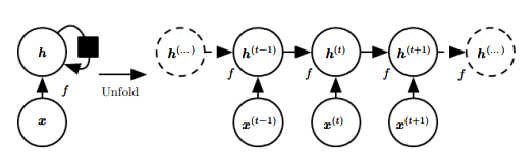
\includegraphics[width=0.8\textwidth]{img/lecture20/h_graph.png}
    \caption{Parameter sharing with state history in sequence models}
    \label{fig:figure_label1}
\end{figure}

\subsection*{Variables in Figure~\ref{fig:figure_label1}}

\begin{itemize}
    \item $\mathbf{x}(t)$: Input vector at time $t$, providing new information at each time step.
    \item $\mathbf{h}(t)$: Hidden state at time $t$, representing the accumulated memory from previous inputs.
    \item $\mathbf{o}(t)$: Output vector at time $t$, generated from the current hidden state.
    \item $\mathbf{U}$: Weight matrix mapping input $\mathbf{x}(t)$ to the hidden state.
    \item $\mathbf{W}$: Weight matrix connecting $\mathbf{h}(t-1)$ to $\mathbf{h}(t)$.
    \item $\mathbf{V}$: Weight matrix mapping $\mathbf{h}(t)$ to the output $\mathbf{o}(t)$.
\end{itemize}

\section{Recurrent Neural Networks (RNNs)}

Recurrent Neural Networks (RNNs) are neural networks designed for sequential data, where the order of inputs is important. As illustrated in Figure~\ref{fig:figure_label2}, RNNs maintain a hidden state that acts as memory, allowing information to persist across time steps. At each time step, the hidden state is updated using both the current input and the previous hidden state, enabling the model to capture temporal dependencies. This makes RNNs well suited for tasks such as language modeling, time-series forecasting, and any application where context from prior inputs influences future predictions.

\subsection{RNN Architecture}\label{subsec:rnn-architecture}

\begin{figure}[H]
    \centering
    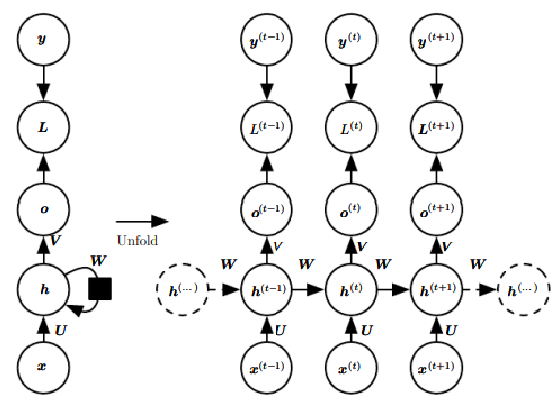
\includegraphics[width=0.8\textwidth]{img/lecture20/bigH.png}
    \caption{The structure of a Recurrent Neural Network (RNN) and how the states and inputs are processed over time}
    \label{fig:figure_label2}
\end{figure}

The key idea behind RNNs is that each output depends not only on the current input but also on a hidden \emph{state} that summarizes past information. Because the same parameters are reused at every time step, RNNs can handle variable-length sequences while keeping the number of parameters manageable.

At a high level, the hidden state evolves according to the recurrence
\[
\mathbf{h}(t) = f(\mathbf{h}(t-1), \mathbf{x}(t)),
\]
where \(f(\cdot)\) is a nonlinear function such as \(\tanh\) or ReLU.

To make this computation explicit, we introduce bias vectors \(\mathbf{b}\) and \(\mathbf{c}\) and write the full RNN update equations:

\begin{align*}
\mathbf{a}(t) &= \mathbf{b} + \mathbf{W}\mathbf{h}(t-1) + \mathbf{U}\mathbf{x}(t) 
&& \text{(pre-activation)} \\
\mathbf{h}(t) &= \tanh(\mathbf{a}(t)) 
&& \text{(hidden state)} \\
\mathbf{o}(t) &= \mathbf{c} + \mathbf{V}\mathbf{h}(t) 
&& \text{(output logits)} \\
\mathbf{y}(t) &= \text{softmax}(\mathbf{o}(t)) 
&& \text{(output probabilities)}
\end{align*}

These equations show how an RNN processes an input sequence by repeatedly updating its hidden state, combining new information with previously stored context, and producing an output at each time step.

% \subsection{Loss Evaluation and Backpropagation}

% In Recurrent Neural Networks (RNNs), training is performed by comparing the predicted output at each time step with the corresponding target. The total loss over a sequence of length $T$ is typically defined as the sum of the per-time-step losses:

% \[
% L = \sum_{t=1}^{T} L(t),
% \]

% where $L(t)$ denotes the loss at time step $t$. Depending on the task, common choices include Mean Squared Error (MSE) for regression and Cross-Entropy Loss for classification.

% \subsection*{Backpropagation Through Time (BPTT)}

% To minimize this sequence loss, RNNs are trained using Backpropagation Through Time (BPTT), which is an extension of standard backpropagation to sequential models. The RNN is first unrolled across the entire sequence, creating a deep computational graph with one layer per time step. Gradients are then computed by applying the chain rule backward through this unfolded network.

% Because each hidden state depends on the previous hidden state, the gradient at a given time step depends not only on the local loss but also on future time steps. This allows the model to adjust parameters by accounting for the cumulative influence of errors across the entire sequence.

% \subsection*{Gradient Calculation}

% During BPTT, gradients of the loss with respect to the parameters (e.g., $\mathbf{U}, \mathbf{W}, \mathbf{V}$) accumulate contributions from all time steps:

% \[
% \frac{\partial L}{\partial \mathbf{W}} 
% = \sum_{t=1}^{T} \frac{\partial L(t)}{\partial \mathbf{W}}.
% \]

% However, computing each term requires repeated application of the chain rule through the hidden state dynamics. For example, gradients with respect to $\mathbf{W}$ involve products of Jacobian matrices of the form

% \[
% \frac{\partial \mathbf{h}(t)}{\partial \mathbf{h}(t-1)},
% \]

% which are multiplied across many time steps.

% \subsection*{Challenges and Solutions}

% Because gradients involve repeated multiplication of these Jacobians, their magnitudes can shrink exponentially (vanishing gradients) or grow exponentially (exploding gradients), particularly in long sequences. Vanishing gradients make it difficult for the network to learn long-range dependencies, while exploding gradients can cause numerical instability during training.

% Common mitigation strategies include gradient clipping to control exploding gradients, and specialized recurrent architectures such as Long Short-Term Memory (LSTM) networks and Gated Recurrent Units (GRUs), which are designed to preserve information over longer time horizons by regulating the flow of gradients.

% In summary, loss evaluation and BPTT enable RNNs to learn temporal dependencies by propagating error signals backward through time and adjusting parameters based on the cumulative sequence-level objective.

% \subsection{The Vanishing Gradient Problem}

% When training Recurrent Neural Networks (RNNs), a major challenge is the \textbf{vanishing gradient problem}, which becomes severe when backpropagating through long sequences. Because RNNs are trained using Backpropagation Through Time (BPTT), gradients must propagate through many time steps of the unrolled network. As a result, the gradient at a given time step depends not only on the local loss but also on contributions from many earlier states.

% During BPTT, gradients with respect to parameters accumulate across time:
% \[
% \frac{\partial \mathcal{L}}{\partial \mathbf{W}}
% = \sum_{t=1}^{T} \frac{\partial L(t)}{\partial \mathbf{W}}.
% \]
% However, computing each term requires repeated application of the chain rule through the hidden-state dynamics.

% \subsection*{Gradient Propagation in RNNs}

% Recall the RNN state update:
% \[
% \mathbf{h}(t)=\sigma\!\left(\mathbf{b}+\mathbf{W}\mathbf{h}(t-1)+\mathbf{U}\mathbf{x}(t)\right).
% \]

% To understand gradient behavior, consider how a hidden state at time \(t\) depends on a much earlier state:
% \[
% \frac{\partial \mathbf{h}(t)}{\partial \mathbf{h}(0)}
% = \prod_{k=1}^{t}\frac{\partial \mathbf{h}(k)}{\partial \mathbf{h}(k-1)}.
% \]

% From the update equation,
% \[
% \frac{\partial \mathbf{h}(t)}{\partial \mathbf{h}(t-1)}
% = \mathbf{J}(t)\mathbf{W}^{T},
% \]
% where \(\mathbf{J}(t)\) is the Jacobian of the activation function \(\sigma\).

% Expanding across time steps gives a long product:
% \[
% \frac{\partial \mathbf{h}(t)}{\partial \mathbf{h}(0)}
% = \mathbf{J}(t)\mathbf{W}^{T}
% \mathbf{J}(t-1)\mathbf{W}^{T}\cdots
% \mathbf{J}(1)\mathbf{W}^{T}.
% \]

% \subsection*{Why Gradients Vanish}

% This expression reveals the core problem: gradients become products of many matrices.  
% If the eigenvalues of \(\mathbf{W}\) (and derivatives of \(\sigma\)) are smaller than 1, repeated multiplication drives the gradient toward zero:
% \[
% \frac{\partial \mathbf{h}(t)}{\partial \mathbf{h}(0)} \approx 0
% \quad \text{for large } t.
% \]

% This makes it difficult for RNNs to learn long-range dependencies.

% \subsection*{Mitigating the Vanishing Gradient Problem}

% Several techniques help preserve gradient flow:

% \begin{itemize}
% \item \textbf{ReLU Activations:} Non-saturating activations maintain larger gradients compared to sigmoid or tanh.
% \item \textbf{Identity Initialization:} Initializing \(\mathbf{W}\) close to the identity matrix stabilizes gradient magnitude across time.
% \item \textbf{Gradient Clipping:} Prevents exploding gradients during training.
% \item \textbf{LSTM and GRU Architectures:} Specially designed gating mechanisms enable long-term memory.
% \end{itemize}

% These improvements allow RNNs to capture longer temporal dependencies.

% \begin{figure}[H]
%     \centering
%     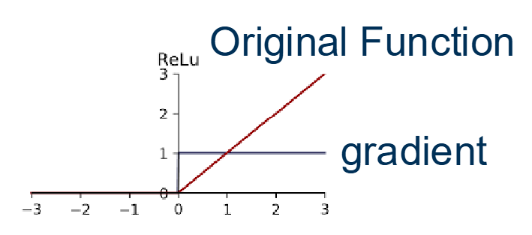
\includegraphics[width=0.8\textwidth]{img/lecture20/Gradient.png}
%     \caption{Effects of standard initialization versus identity initialization}
%     \label{fig:figure_label3}
% \end{figure}

% \begin{figure}[H]
%     \centering
%     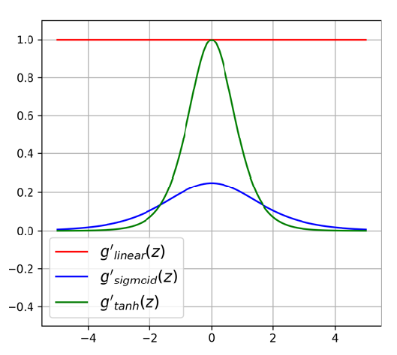
\includegraphics[width=0.8\textwidth]{img/lecture20/ReLU.png}
%     \caption{Comparison of sigmoid, tanh, and ReLU activation functions}
%     \label{fig:figure_label4}
% \end{figure}

\subsection{Loss Evaluation and Backpropagation}

In RNN training, the predicted output at each time step is compared with the corresponding target output. The total loss over a sequence of length \(T\) is typically defined as the sum of per-time-step losses:
\[
\mathcal{L} = \sum_{t=1}^{T} L(t),
\]
where \(L(t)\) denotes the loss at time step \(t\). Common choices include Mean Squared Error (MSE) for regression and Cross-Entropy Loss for classification.

To minimize this sequence-level objective, RNNs are trained using \textbf{Backpropagation Through Time (BPTT)}, an extension of standard backpropagation for sequential models. The network is first \emph{unrolled} across the entire sequence, forming a deep computational graph with one layer per time step. Gradients are then computed by applying the chain rule backward through this unfolded network.

Because each hidden state depends on the previous hidden state, the gradient at a given time step depends not only on the local loss but also on future time steps. During BPTT, gradients with respect to the parameters (e.g., \( \mathbf{U}, \mathbf{W}, \mathbf{V} \)) accumulate contributions from the entire sequence:
\[
\frac{\partial \mathcal{L}}{\partial \mathbf{W}} 
= \sum_{t=1}^{T} \frac{\partial L(t)}{\partial \mathbf{W}}.
\]

However, computing each term requires repeated application of the chain rule through the hidden-state dynamics. In particular, gradients with respect to the recurrent weights involve products of Jacobian matrices of the form
\[
\frac{\partial \mathbf{h}(t)}{\partial \mathbf{h}(t-1)},
\]
which are multiplied across many time steps. This repeated multiplication leads directly to a fundamental training challenge for RNNs.

\subsection{The Vanishing Gradient Problem}

A major difficulty in training RNNs is the \textbf{vanishing gradient problem}, which becomes severe when backpropagating through long sequences. Because BPTT requires gradients to propagate across many time steps, small changes in gradient magnitude can compound dramatically.

\subsection*{Gradient Propagation in RNNs}

As introduced in Section~\ref{subsec:rnn-architecture}, the RNN state update is
\[
\mathbf{a}(t)=\mathbf{b}+\mathbf{W}\mathbf{h}(t-1)+\mathbf{U}\mathbf{x}(t),
\qquad
\mathbf{h}(t)=\sigma(\mathbf{a}(t)),
\]
where \(\sigma(\cdot)\) is an element-wise nonlinearity (e.g., \(\tanh\) or ReLU).

To understand gradient behavior, consider how a hidden state at time \(t\) depends on a much earlier state:
\[
\frac{\partial \mathbf{h}(t)}{\partial \mathbf{h}(0)}
= \prod_{k=1}^{t}\frac{\partial \mathbf{h}(k)}{\partial \mathbf{h}(k-1)}.
\]

From the update equation,
\[
\frac{\partial \mathbf{h}(t)}{\partial \mathbf{h}(t-1)}
= \mathbf{J}(t)\mathbf{W}^{T},
\]
where \(\mathbf{J}(t)=\mathrm{diag}\!\left(\sigma'(\mathbf{a}(t))\right)\) is the Jacobian of the activation function.

Expanding across time steps yields
\[
\frac{\partial \mathbf{h}(t)}{\partial \mathbf{h}(0)}
= \mathbf{J}(t)\mathbf{W}^{T}
\mathbf{J}(t-1)\mathbf{W}^{T}\cdots
\mathbf{J}(1)\mathbf{W}^{T}.
\]

\subsection*{Why Gradients Vanish}

Gradients therefore become products of many matrices. If the eigenvalues of \(\mathbf{W}\) and the derivatives of the activation function are smaller than one, repeated multiplication drives the gradient toward zero:
\[
\frac{\partial \mathbf{h}(t)}{\partial \mathbf{h}(0)} \approx 0
\quad \text{for large } t.
\]

As a result, early time steps have little influence on learning, making it difficult for RNNs to capture long-range dependencies.

\subsection*{Mitigating the Vanishing Gradient Problem}

Several techniques help preserve gradient flow:

\begin{itemize}
\item \textbf{ReLU activations:} Non-saturating activations maintain larger gradients than sigmoid or tanh.
\item \textbf{Identity initialization:} Initializing \(\mathbf{W}\) close to the identity stabilizes gradient magnitude across time.
\item \textbf{Gradient clipping:} Prevents exploding gradients during training.
\item \textbf{LSTM and GRU architectures:} Gating mechanisms enable long-term memory.
\end{itemize}

These improvements allow RNNs to capture longer temporal dependencies.

\begin{figure}[H]
    \centering
    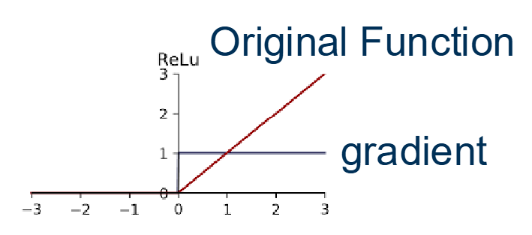
\includegraphics[width=0.8\textwidth]{img/lecture20/Gradient.png}
    \caption{Effects of standard initialization versus identity initialization}
    \label{fig:figure_label3}
\end{figure}

\begin{figure}[H]
    \centering
    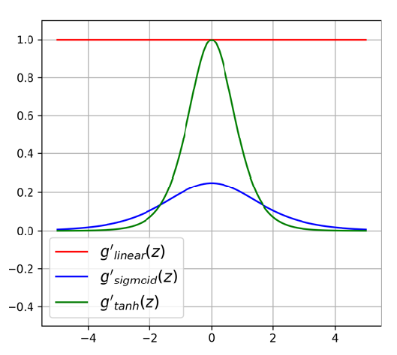
\includegraphics[width=0.8\textwidth]{img/lecture20/ReLU.png}
    \caption{Comparison of sigmoid, tanh, and ReLU activation functions}
    \label{fig:figure_label4}
\end{figure}

\section{Long Short-Term Memory (LSTM) Networks}

Long Short-Term Memory (LSTM) networks are a type of Recurrent Neural Network (RNN) specifically designed to address the vanishing gradient problem discussed in Section~\ref{subsec:rnn-architecture}. By introducing a memory cell and a set of gating mechanisms, LSTMs regulate the flow of information through time and enable learning of long-term dependencies. Figure~\ref{fig:figure_label5} illustrates the structure of an individual LSTM cell.

\begin{figure}[H]
    \centering
    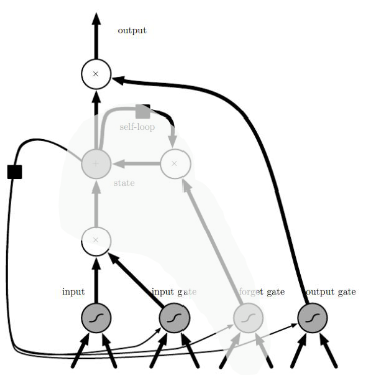
\includegraphics[width=0.8\textwidth]{img/lecture20/LSTM.png}
    \caption{An LSTM cell for one time step}
    \label{fig:figure_label5}
\end{figure}

\subsection{LSTM Architecture and Gates}

An LSTM cell augments the standard RNN hidden state with a \textbf{cell state} that serves as long-term memory. Information is regulated through three multiplicative gates that decide what to forget, what to store, and what to output at each time step.

\begin{itemize}
    \item \textbf{Forget Gate} \( \mathbf{f}^{(t)} \):  
    Determines how much of the previous cell state should be retained:
    \[
    \mathbf{f}^{(t)} 
    = \sigma(\mathbf{b}^f + \mathbf{U}^f \mathbf{x}^{(t)} + \mathbf{W}^f \mathbf{h}^{(t-1)})
    \]

    \item \textbf{Input Gate} \( \mathbf{g}^{(t)} \):  
    Controls how much new information should be written to memory:
    \[
    \mathbf{g}^{(t)} 
    = \sigma(\mathbf{b}^g + \mathbf{U}^g \mathbf{x}^{(t)} + \mathbf{W}^g \mathbf{h}^{(t-1)})
    \]

    \item \textbf{Output Gate} \( \mathbf{o}^{(t)} \):  
    Determines which parts of the memory influence the hidden state:
    \[
    \mathbf{o}^{(t)} 
    = \sigma(\mathbf{b}^o + \mathbf{U}^o \mathbf{x}^{(t)} + \mathbf{W}^o \mathbf{h}^{(t-1)})
    \]
\end{itemize}

\subsection{Updating the Cell and Hidden States}

After computing the gates, the LSTM updates its internal memory and hidden state in three steps.

\begin{itemize}

\item \textbf{Candidate Cell State:}
\[
\tilde{\mathbf{s}}^{(t)} 
= \tanh(\mathbf{b}^c + \mathbf{U}^c \mathbf{x}^{(t)} + \mathbf{W}^c \mathbf{h}^{(t-1)})
\]

\item \textbf{Cell State Update:}
\[
\mathbf{s}^{(t)} 
= \mathbf{f}^{(t)} \circ \mathbf{s}^{(t-1)} 
+ \mathbf{g}^{(t)} \circ \tilde{\mathbf{s}}^{(t)}
\]

\item \textbf{Hidden State Update:}
\[
\mathbf{h}^{(t)} 
= \mathbf{o}^{(t)} \circ \tanh(\mathbf{s}^{(t)})
\]

\end{itemize}

Here, \( \circ \) denotes element-wise multiplication.  
This additive memory update allows gradients to flow more easily across time steps, mitigating the vanishing gradient problem.

\subsection{Advantages of LSTMs over Standard RNNs}

LSTMs are highly effective for modeling long sequences because their gated memory structure allows information to persist across many time steps. The additive update of the cell state provides a stable pathway for gradients, significantly reducing the vanishing gradient problem that affects standard RNNs. As a result, LSTMs can selectively remember or forget information, making them well suited for tasks such as natural language processing, speech recognition, and time-series forecasting.

\subsection{Limitations of LSTMs}

Despite their strengths, LSTMs also have several practical drawbacks. Their gating mechanisms introduce multiple weight matrices, increasing computational cost and the number of trainable parameters compared to standard RNNs. This can lead to slower training and a greater risk of overfitting on smaller datasets. In addition, like all recurrent architectures, LSTMs process sequences sequentially, limiting opportunities for parallel computation. For large-scale sequence modeling, modern Transformer architectures often provide better scalability and performance.

\section{Gated Recurrent Units (GRUs)}

Gated Recurrent Units (GRUs) are a recurrent neural network architecture designed as a simpler alternative to Long Short-Term Memory (LSTM) networks. GRUs capture long-range dependencies in sequential data while using fewer parameters and a more streamlined structure. This efficiency is achieved by combining the forget and input gates of LSTMs into a single update gate and eliminating the separate cell state, relying instead on a single hidden state.

\subsection{GRU Architecture and Gates}

Each GRU cell contains two gates that regulate information flow:

\begin{itemize}
    \item \textbf{Update Gate} \( \mathbf{z}^{(t)} \): controls how much of the previous hidden state is preserved:
    \[
    \mathbf{z}^{(t)}=\sigma(\mathbf{b}^z+\mathbf{U}^z\mathbf{x}^{(t)}+\mathbf{W}^z\mathbf{h}^{(t-1)})
    \]

    \item \textbf{Reset Gate} \( \mathbf{r}^{(t)} \): determines how much past information to forget when forming the candidate state:
    \[
    \mathbf{r}^{(t)}=\sigma(\mathbf{b}^r+\mathbf{U}^r\mathbf{x}^{(t)}+\mathbf{W}^r\mathbf{h}^{(t-1)})
    \]
\end{itemize}

\subsection{Updating the Hidden State}

Using these gates, the GRU first computes a candidate hidden state
\[
\tilde{\mathbf{h}}^{(t)}=\tanh\!\left(\mathbf{b}+\mathbf{U}\mathbf{x}^{(t)}+\mathbf{W}(\mathbf{r}^{(t)}\circ\mathbf{h}^{(t-1)})\right),
\]
which incorporates the reset gate to control how much past information is used.

The final hidden state is then obtained by interpolating between the previous hidden state and the candidate state:
\[
\mathbf{h}^{(t)}=\mathbf{z}^{(t)}\circ\mathbf{h}^{(t-1)}+(1-\mathbf{z}^{(t)})\circ\tilde{\mathbf{h}}^{(t)}.
\]

This gating mechanism enables GRUs to adaptively preserve or update memory over time.

\subsection{Advantages of GRUs}

GRUs are computationally efficient due to their simpler architecture and reduced number of parameters compared to LSTMs. This often leads to faster training and lower memory usage while still capturing long-term dependencies in sequential data. In practice, GRUs frequently achieve performance comparable to LSTMs on many sequence modeling tasks, making them attractive when computational resources are limited.

\subsection{Limitations of GRUs}

Despite their efficiency, GRUs offer less expressive control over memory than LSTMs because they lack a separate cell state. For complex tasks requiring very long-term memory or fine-grained control of information flow, LSTMs may still provide superior performance. As with other recurrent models, GRUs also process sequences sequentially, limiting parallelization and scalability compared to Transformer architectures.

\subsection{Parameter Sharing in Sequence Modeling}

A key strength of recurrent models such as RNNs, LSTMs, and GRUs is parameter sharing across time steps. The same weight matrices are reused at every position in a sequence, allowing the model to process inputs of varying lengths without increasing the number of parameters.

This idea is closely related to parameter sharing in Convolutional Neural Networks (CNNs), where the same convolutional kernel is applied across different spatial locations. Parameter sharing provides two major benefits. First, it enables the detection of patterns regardless of their position in the sequence, leading to invariance. Second, it allows efficient modeling of variable-length inputs without increasing model size.

\begin{figure}[H]
    \centering
    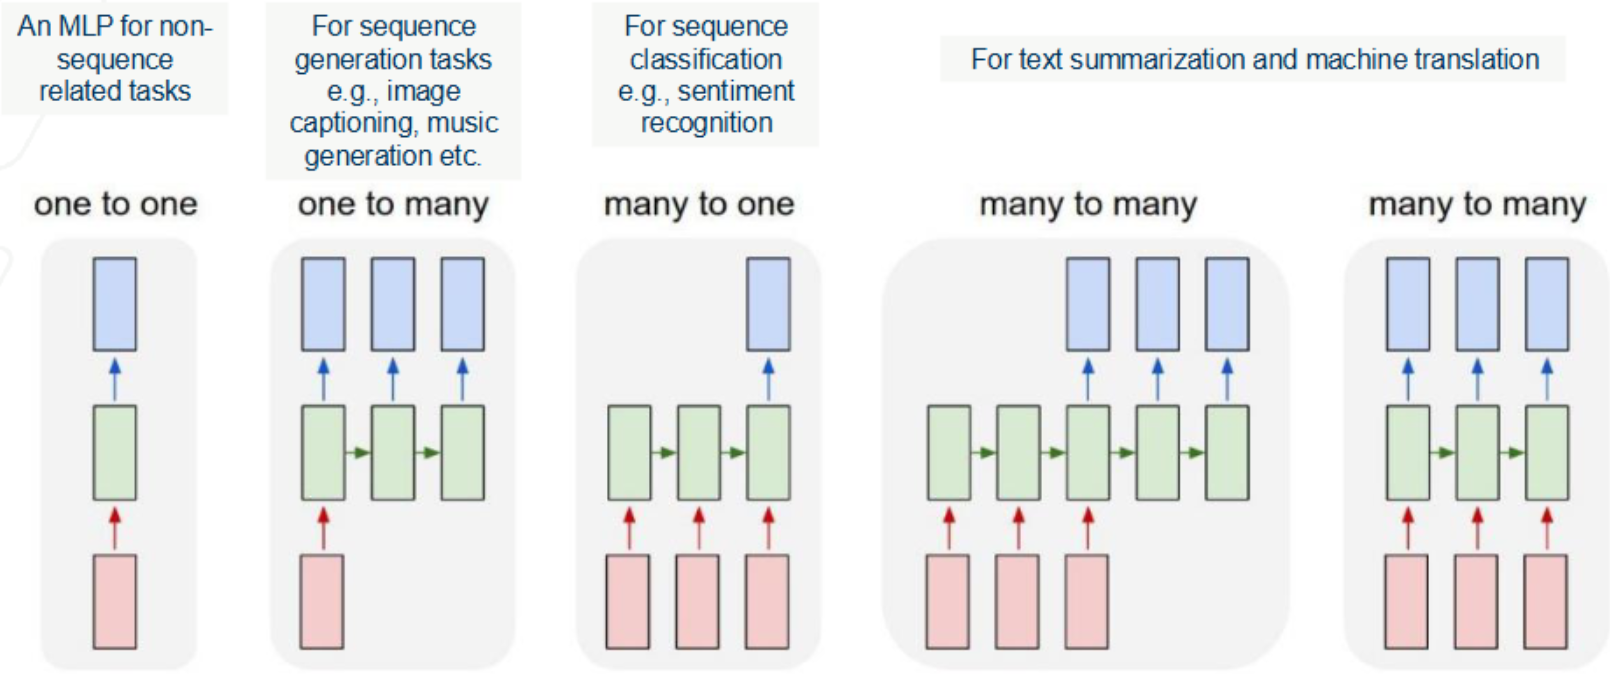
\includegraphics[width=0.8\textwidth]{img/lecture20/RNN_Config.png}
    \caption{Various configurations for RNNs and related sequence models. Blue boxes denote outputs, red boxes inputs, and green boxes hidden states.}
    \label{fig:figure_label6}
\end{figure}

% \section{Temporal Convolutional Networks (TCNs)}

% Temporal Convolutional Networks (TCNs) are convolution-based architectures designed for sequence modeling. Unlike recurrent models such as RNNs, LSTMs, and GRUs, TCNs replace recurrence with one-dimensional convolutions applied along the temporal dimension. By leveraging convolutional layers, TCNs process entire sequences in parallel, enabling efficient computation while maintaining the ability to capture long-range temporal dependencies.

% \subsection{Motivation for TCNs}

% Recurrent neural networks suffer from several practical limitations. Their sequential processing prevents parallelization across time steps, leading to computational bottlenecks for long sequences. In addition, gradients must propagate through many time steps, which can result in vanishing or exploding gradient behavior. Although architectures such as LSTMs and GRUs mitigate these issues, they still rely on sequential computation.

% TCNs address these challenges by replacing recurrence with causal, dilated convolutions. This allows parallel processing across time while maintaining strict temporal ordering.

% \subsection{Computation in TCNs}

% A TCN consists of stacked one-dimensional convolutional layers applied along the time axis. Each layer produces an output sequence of the same length as the input sequence. Because convolutions are applied simultaneously across all time steps, training and inference can be parallelized.

% Stacking multiple convolutional layers increases the receptive field of the network. Deeper layers can therefore model longer temporal dependencies without requiring recurrent connections. Figure~\ref{fig:figure_label10} illustrates how stacking layers expands the receptive field.

% \subsection{Core Components of TCNs}

% Modern TCN architectures rely on three key design principles:

% \subsubsection*{Causal Convolutions}

% Causal convolutions ensure that the output at time \( t \) depends only on inputs from time \( t \) and earlier. This preserves temporal ordering and prevents leakage of future information.

% For a kernel of length \( k \), the convolution at time \( t \) is given by

% \[
% \mathbf{y}^{(t)} = f\left(\mathbf{x}^{(t)}, \mathbf{x}^{(t-1)}, \dots, \mathbf{x}^{(t-k+1)}\right).
% \]

% To preserve sequence length, the input is padded with \( k-1 \) zeros on the left. Figures~\ref{fig:figure_label7}--\ref{fig:figure_label9} illustrate the padding and convolution process.

% Causal convolutions make TCNs suitable for forecasting and real-time prediction tasks, where future information must not influence current outputs.

% \subsubsection*{Dilated Convolutions}

% While standard convolutions increase the receptive field linearly with depth, dilated convolutions expand it exponentially without increasing parameter count.

% A dilated convolution with kernel size \( k \) and dilation factor \( d \) is defined as

% \[
% \mathbf{y}^{(t)} = f\left(\mathbf{x}^{(t)}, \mathbf{x}^{(t-d)}, \dots, \mathbf{x}^{(t-d(k-1))}\right).
% \]

% The dilation factor typically grows with depth (e.g., \( d = 1, 2, 4, 8, \dots \)), allowing deeper layers to access exponentially larger temporal contexts. Figures~\ref{fig:figure_label13} and \ref{fig:figure_label14} demonstrate how dilation expands the receptive field by skipping intermediate time steps.

% \subsubsection*{Residual Connections}

% To enable stable training of deep TCNs, residual connections are incorporated into each convolutional block. A residual block adds the input directly to the block output, forming a shortcut path for gradients.

% A simplified residual block can be written as

% \[
% \mathbf{h}^{(t)} = \mathbf{x}^{(t)} + \phi\!\left(W_2 \, \phi\!\left(W_1 \mathbf{x}^{(t)} + \mathbf{b}_1\right) + \mathbf{b}_2\right),
% \]

% where \( \phi(\cdot) \) is typically a ReLU activation. The residual connection improves gradient flow and prevents degradation in very deep networks. Figure~\ref{fig:figure_label16} shows the structure of a residual block in a TCN.

% \subsection{Computational Complexity}

% One of the primary advantages of TCNs over recurrent models is their computational scalability. Because convolutions operate across all time steps simultaneously, TCNs allow parallel computation during training and inference.

% For a sequence of length \( T \), kernel size \( k \), and \( F \) filters, the complexity per layer is approximately \( \mathcal{O}(T k F) \). Unlike RNNs, computation does not scale sequentially with time in a recursive manner. This makes TCNs particularly effective for long sequences.

% Figures~\ref{fig:figure_label14} and \ref{fig:figure_label15} illustrate how stacked dilated convolutions expand the receptive field without increasing per-layer computational cost significantly.

% \subsection{Advantages of TCNs}

% TCNs offer several advantages over recurrent architectures:

% First, they enable full parallelization across time steps, resulting in faster training and inference. Second, causal convolutions ensure proper temporal ordering, making them well suited for forecasting tasks. Third, dilated convolutions allow TCNs to model long-range dependencies with relatively shallow depth. Finally, residual connections facilitate stable optimization of deep architectures.

% In practice, TCNs often outperform recurrent models on long-sequence benchmarks due to their efficient receptive field design and improved gradient behavior.

% \subsection{Limitations of TCNs}

% Despite their strengths, TCNs also have limitations. The receptive field is fixed once the architecture is defined, meaning that extremely long dependencies may require deeper networks or larger dilation factors. Additionally, convolutional filters may struggle with tasks that require adaptive memory mechanisms, where recurrent gating can provide finer control.

% Furthermore, while TCNs parallelize well, their memory usage can increase with depth due to storing intermediate activations across all time steps.

% \subsection{Weight Normalization}

% Weight normalization is often applied in TCN layers to stabilize training. It reparameterizes the weight vector \( \mathbf{w} \) as

% \[
% \mathbf{w} = \frac{\mathbf{g}}{\|\mathbf{v}\|} \mathbf{v},
% \]

% where \( \mathbf{v} \) represents the original weight vector and \( \mathbf{g} \) is a learnable scalar parameter. This separation of magnitude and direction helps maintain stable gradient magnitudes across layers, improving convergence in deep convolutional stacks.

% \section{Appendix: Notations}
% \begin{itemize}
%     \item \( x_i \): Single feature
%     \item \( \mathbf{x}_i \): Feature vector (data sample)
%     \item \( \mathbf{X} \): Matrix of feature vectors (dataset)
%     \item \( W \): Weight matrix
%     \item \( P \): Number of features in a feature vector
%     \item \( \alpha \): Learning rate
% \end{itemize}


\section{Q\&A Section}

\begin{enumerate}
    \item \textbf{Question:} 
    Why are standard MLPs poorly suited for sequence modeling, especially when sequence lengths vary?

    \textbf{Solution:}
    MLPs assume \emph{fixed-size} inputs and outputs, so they do not naturally handle variable-length sequences. More importantly, an MLP processes inputs as independent feature vectors, so it does not encode temporal order and cannot capture dependencies across time. Modeling long sequences with an MLP typically requires a large number of parameters (e.g., by concatenating many time steps into one huge input), which increases memory/computation and often leads to overfitting when data is limited.

    \item \textbf{Question:}
    Write the forward-pass equations of a basic RNN (with bias terms) that produces a probability vector at each time step.

    \textbf{Solution:}
    A standard RNN computes, for each time step $t$:
    \[
    \mathbf{a}(t)=\mathbf{b}+\mathbf{W}\mathbf{h}(t-1)+\mathbf{U}\mathbf{x}(t),
    \qquad
    \mathbf{h}(t)=\tanh(\mathbf{a}(t)),
    \]
    then outputs logits and probabilities:
    \[
    \mathbf{o}(t)=\mathbf{c}+\mathbf{V}\mathbf{h}(t),
    \qquad
    \mathbf{y}(t)=\mathrm{softmax}(\mathbf{o}(t)).
    \]

    \item \textbf{Question:}
    In Backpropagation Through Time (BPTT), why can gradients \emph{vanish} as the sequence length grows? Give the key product form that explains this behavior.

    \textbf{Solution:}
    In BPTT, the dependence of a later hidden state on an earlier hidden state contains a product of Jacobians:
    \[
    \frac{\partial \mathbf{h}(t)}{\partial \mathbf{h}(0)}
    =\prod_{k=1}^{t}\frac{\partial \mathbf{h}(k)}{\partial \mathbf{h}(k-1)}.
    \]
    For the RNN update $\mathbf{h}(t)=\sigma(\mathbf{a}(t))$ with $\mathbf{a}(t)=\mathbf{b}+\mathbf{W}\mathbf{h}(t-1)+\mathbf{U}\mathbf{x}(t)$,
    \[
    \frac{\partial \mathbf{h}(t)}{\partial \mathbf{h}(t-1)}=\mathbf{J}(t)\mathbf{W}^T,
    \quad \text{where } \mathbf{J}(t)=\mathrm{diag}(\sigma'(\mathbf{a}(t))).
    \]
    Thus,
    \[
    \frac{\partial \mathbf{h}(t)}{\partial \mathbf{h}(0)}
    =\mathbf{J}(t)\mathbf{W}^T\mathbf{J}(t-1)\mathbf{W}^T\cdots \mathbf{J}(1)\mathbf{W}^T.
    \]
    If the relevant singular values/eigenvalues of $\mathbf{W}$ and typical magnitudes of $\sigma'(\cdot)$ are $<1$, repeated multiplication shrinks the gradient exponentially toward $0$, making early time steps contribute very little to learning.

    \item \textbf{Question:}
    State the LSTM gate equations (forget, input, output), and the update equations for the cell state and hidden state. What is the key structural reason LSTMs reduce vanishing gradients?

    \textbf{Solution:}
    The gates are:
    \[
    \mathbf{f}^{(t)}=\sigma(\mathbf{b}^f+\mathbf{U}^f\mathbf{x}^{(t)}+\mathbf{W}^f\mathbf{h}^{(t-1)}),\quad
    \mathbf{g}^{(t)}=\sigma(\mathbf{b}^g+\mathbf{U}^g\mathbf{x}^{(t)}+\mathbf{W}^g\mathbf{h}^{(t-1)}),
    \]
    \[
    \mathbf{o}^{(t)}=\sigma(\mathbf{b}^o+\mathbf{U}^o\mathbf{x}^{(t)}+\mathbf{W}^o\mathbf{h}^{(t-1)}).
    \]
    Candidate cell state, cell update, and hidden update:
    \[
    \tilde{\mathbf{s}}^{(t)}=\tanh(\mathbf{b}^c+\mathbf{U}^c\mathbf{x}^{(t)}+\mathbf{W}^c\mathbf{h}^{(t-1)}),
    \]
    \[
    \mathbf{s}^{(t)}=\mathbf{f}^{(t)}\circ \mathbf{s}^{(t-1)}+\mathbf{g}^{(t)}\circ \tilde{\mathbf{s}}^{(t)},\quad
    \mathbf{h}^{(t)}=\mathbf{o}^{(t)}\circ\tanh(\mathbf{s}^{(t)}).
    \]
    Key reason: the cell state update is \emph{additive} (a controlled “skip” pathway through time), which provides a more stable route for gradient flow compared to repeatedly multiplying by $\mathbf{W}$ and $\sigma'(\cdot)$ at every step.

    % \item \textbf{Question:}
    % What makes a Temporal Convolutional Network (TCN) \emph{causal}, and how do \emph{dilated convolutions} help it model long-range dependencies efficiently?

    % \textbf{Solution:}
    % A TCN is causal if the output at time $t$ depends only on inputs at times $\le t$ (no future leakage). With a kernel length $k$:
    % \[
    % \mathbf{y}^{(t)} = f\!\left(\mathbf{x}^{(t)},\mathbf{x}^{(t-1)},\dots,\mathbf{x}^{(t-k+1)}\right),
    % \]
    % typically implemented by left-padding the input so the convolution never accesses future indices.
    % Dilated convolutions expand the receptive field without increasing parameter count by skipping inputs with dilation factor $d$:
    % \[
    % \mathbf{y}^{(t)} = f\!\left(\mathbf{x}^{(t)},\mathbf{x}^{(t-d)},\dots,\mathbf{x}^{(t-d(k-1))}\right).
    % \]
    % Using dilation factors like $d=1,2,4,8,\dots$ across stacked layers grows the receptive field roughly exponentially with depth, enabling long-range temporal modeling while keeping per-layer computation comparable to standard convolutions.
    
    \item \textbf{Question:}
    Compare \textbf{RNNs}, \textbf{LSTMs} and \textbf{GRUs} in terms of (i) ability to model long-range dependencies, (ii) parameter/computational cost, and (iii) parallelizability.
    
   \textbf{Solution:}
    \begin{itemize}
        \item \textbf{RNNs:}
        The simplest recurrent models. They often struggle with long-range dependencies due to vanishing/exploding gradients. They use fewer parameters than gated variants but process sequences sequentially, limiting parallelism across time.
    
        \item \textbf{LSTMs:}
        Introduce a separate cell state and multiple gates to stabilize gradient flow and improve long-range modeling. They require more parameters and computational cost than vanilla RNNs and still operate sequentially.
    
        \item \textbf{GRUs:}
        A streamlined alternative to LSTMs that combines gates and removes the separate cell state. They often achieve similar performance with fewer parameters and faster training, but remain sequential due to recurrence.
    
        % \item \textbf{TCNs:}
        % Replace recurrence with 1D causal and dilated convolutions. They process all time steps in parallel within each layer, enabling faster training. Long-range dependencies are modeled via expanded receptive fields (through dilation). However, the maximum dependency length is limited by depth, kernel size, and dilation schedule.
    \end{itemize}
    
    % \item \textbf{Question:}
    % (\textbf{Dilated TCN receptive field}) Consider a TCN with \textbf{3} causal 1D convolution layers, kernel size $k=3$, and dilation factors $d_1=1$, $d_2=2$, $d_3=4$. Assuming stride $1$ and that each layer preserves sequence length (via causal padding), how many past time steps (including the current time step) can influence the output at time $t$ in the final layer?
    
    % \textbf{Solution:}
    % For a stack of causal dilated convolutions (stride $1$), the receptive field length is
    % \[
    % R \;=\; 1 + \sum_{\ell=1}^{L} (k-1)\,d_\ell.
    % \]
    % Here $L=3$, $k=3$, so $(k-1)=2$, and $d_1=1$, $d_2=2$, $d_3=4$. Thus,
    % \[
    % R \;=\; 1 + 2(1+2+4) \;=\; 1 + 2\cdot 7 \;=\; 15.
    % \]
    % So the output at time $t$ can depend on inputs from times $t, t-1, \dots, t-14$ (a total of $15$ time steps).
        
\end{enumerate}


\end{document}